\documentclass[10pt,a4paper]{beamer}
\usepackage[utf8]{inputenc}
\usepackage[english]{babel}
\usepackage{amsmath}
\usepackage{amsfonts}
\usepackage{amssymb}
\usepackage{listings}
\usepackage{hyperref}
\usepackage{graphicx}
\usepackage{listings}
\usepackage{mathpartir}
\usepackage{hyperref}
\hypersetup{colorlinks,urlcolor=blue}

\usetheme{Warsaw}

\lstset
{
	basicstyle = \ttfamily\footnotesize,
	breaklines = true,
	frame = single
}

\begin{document}

\author[Di Giacomo et al.]
{Francesco ~Di Giacomo \inst{1} \\
	\and Mohamed ~Abbadi \inst{3} \\
	\and Agostino ~Cortesi \inst{1} \\
	\and Pieter ~Spronck \inst{2} \\
	\and Giuseppe ~Maggiore \inst{3}}
\institute[Universities Here and There] % (optional)
{
  Università Ca' Foscari - Venice
  \and Tilburg University - Tilburg
  \and Hogeschool Rotterdam - Rotterdam
}
\date{}
\title{Metacasanova: An Optimized Meta-compiler for Domain-Specific Languages}

\frame{\titlepage}

\begin{frame}
\frametitle{Summary}

We present Metacasanova, a meta-compiler initially created to ease the development of Casanova, a DSL for game development.

\vspace{1cm}
\textbf{Topics:}
\begin{itemize}
	\item Introduction on DSL.
	\item Introduction of Metacasanova and example of use.
	\item Language extension with Functors.
	\item Example of Records implemented with Functors.
	\item Results and Conclusion.
\end{itemize}
\end{frame}


\begin{frame}
\frametitle{Domain-Specific Languages}
\framesubtitle{Advantages of DSL's}
\begin{itemize}
	\item Abstractions that are closer to the problem domain.
	\item Speed-up of development time of the problem solution.	
\end{itemize}
\end{frame}

\begin{frame}
\frametitle{Domain-Specific Languages}
\framesubtitle{DSL's implementation}

Two possible paths:

\begin{enumerate}
	\item Embed the DSL in a host language.
	\item Write a compiler/interpreter.
\end{enumerate}

\textbf{Embedding Pros and Cons:}

\begin{itemize}
	\item Re-use of the host language infrastructure.
	\item Developers expert in the host-language need only to become familiar with the language extension.
	\item Syntax and type system bound to those of the host language. Type system as well.
	\item Domain-specific optimizations are difficult.
\end{itemize}

\textbf{Compilation/interpretation Pros and Cons}

\begin{itemize}
	\item Syntax and types correspond to the language definition.
	\item Good error reporting.
	\item Domain-specific optimizations are possible.
	\item Long development time.
	\item Development process follows recurrent patterns.
\end{itemize}
\end{frame}

\begin{frame}
\frametitle{Domain-Specific Languages}
\framesubtitle{Steps in Compilers Development}
\begin{enumerate}
	\item Formalize the grammar of the language.
	\item Formalize the type system and semantics.
	\item Build a syntactical analyser.
	\item Build a type checker.
	\item Implement the semantics in the target language.
\end{enumerate}
\end{frame}

\begin{frame}
\frametitle{Domain-Specific Languages}
\framesubtitle{Steps in Compilers Development - Recurring steps}
\begin{itemize}
	\item Step 1 and 2 are creative and cannot be captured by a pattern.
	\item Step 3 can be completed by using a Lexer/Parser generator.
	\item Step 4 processes the result of the syntax analysis and implements the formalization of the type system in a chosen programming language.
	\item Step 5 takes the result of Step 4 and implements the formalization of the semantics in the target language.
\end{itemize}

Step 4 and 5 are independent of the language we are building the compiler for.
\end{frame}

\begin{frame}
\frametitle{Domain-Specific Languages}
\framesubtitle{Steps in Compilers Development - Problems}
\begin{itemize}
	\item The formalization of the types and semantics is lost when implemented with the abstraction of the chosen programming language.
	\item The implementation mimics the behaviour of the meta-representation of the formal semantics.
	\item Example: if we use inference rules, then we re-implement their behaviour in the host language each time we write a new compiler.
\end{itemize}

\textbf{Goal:} Express the repetitive steps in terms of the formalization.
\end{frame}

\begin{frame}
\frametitle{Research questions}
\textbf{Research question 1:} \textit{To what extent does Metacasanova ease the development speed of a compiler for a Domain-Specific Language, in terms of code length compared to the hard-coded implementation, and how much does the abstraction layer of the Metacompiler affect the performance of the generated code?}
\pause

\vspace{0.2cm}
\noindent
\textbf{Research question 2:} \textit{In what way can we embed the type system of the implemented language in Metacasanova in order to get rid of the dynamic lookups at runtime and what is the performance gain of this optimization?}
\end{frame}

\begin{frame}
\frametitle{Metacompilation}
\framesubtitle{Metacasanova}

\textbf{Metacompilers}
\begin{itemize}
	\item Input: the definition of a language in a meta-language.
	\item Input: a program written in that language.
	\item Output: Executable code for the program.
\end{itemize}

\textbf{Metacasanova}
\begin{itemize}
	\item Input: Language definition in terms of inference rules.
	\item Input: A meta-representation of the program in that language.
	\item Output: C\# code (it can later be compiled using a .NET compiler).
\end{itemize}
\end{frame}

\begin{frame}
\frametitle{Metacasanova}
\framesubtitle{Meta-program Structure}

\begin{itemize}
	\item Meta-data structure declarations: used to represent the abstractions of the language.
	\item Function declaration: used to process inference rules.
	\item Sub-typing. Used to define different ``roles'' for meta-data structures. For example you can say that an atomic value can be also used as an arithmetic expression.
	\item Inference rules.
	\item It is possible to embed types and methods from an external language.
\end{itemize}
\end{frame}

\begin{frame}
\frametitle{Metacasanova}
\framesubtitle{Semantics of rule evaluation}

\begin{mathpar}
	\mprset{flushleft}
	\inferrule*[left=R1:]
	{C = \emptyset \\\\ F = \emptyset}
	{\langle f^{r} \rangle \Rightarrow \lbrace x \rbrace} \\
	
	\mprset{flushleft}
	\inferrule*[left=R2:]
	{\forall c_{i} \in C \;, \langle c_{i} \rangle \Rightarrow true \\\\
		\forall f_{j} \in F \; , \exists r_{k} \in R \; | \; \langle f_{j}^{r_{k}} \rangle \Rightarrow \lbrace x_{r^{k}} \rbrace}
	{\langle f^{r} \rangle \Rightarrow \lbrace x_{r} \rbrace} \\
	
	\mprset{flushleft}
	\inferrule*[left=R3(a):]
	{\exists c_{i} \in C \; | \; \langle c_{i} \rangle \Rightarrow false}
	{\langle f^{r} \rangle \Rightarrow \emptyset} \\
	
	\mprset{flushleft}
	\inferrule*[left=R3(b)]
	{\forall r_{k} \in R \; , \exists f_{j} \in F \; | \; \langle f_{j}^{r_{k}} \rangle \Rightarrow \emptyset}
	{\langle f^{r} \rangle \Rightarrow \emptyset}
\end{mathpar}

\end{frame}

\begin{frame}[fragile]
\frametitle{Metacasanova}
\framesubtitle{Example: Control structures}
\begin{itemize}
	\item We assume we have meta-data structures representing values in our language.
	\item We assume we already have defined expression evaluations for brevity.
	\item The memory is represented as a meta-data structures containing a map between Id's and values.	
	\begin{lstlisting}
Data "$m" << ImmutableDictionary<Id, Value> >> : SymbolTable
	\end{lstlisting}
	\item We represent local scopes through a list of symbol tables.
	\begin{lstlisting}
Data SymbolTable -> "::" -> TableList : TableList
	\end{lstlisting}
\end{itemize}
\end{frame}

\begin{frame}[fragile]
\frametitle{Metacasanova}
\framesubtitle{Example: Control structures}
\textbf{Meta-data definition of If-Then-Else:}
\begin{lstlisting}
Data "then" : Then
Data "else" : Else
Data "if" -> Expr -> Then -> Stmt -> Else -> Stmt : Stmt
\end{lstlisting}

\textbf{Meta-data definition of While-Do:}
\begin{lstlisting}
Data "do" : Do
Data "while" -> Expr -> Do -> Stmt : Stmt
\end{lstlisting}

\textbf{Evaluation function:}
\begin{lstlisting}
Func "eval" -> TableList -> Stmt : EvaluationResult
\end{lstlisting}
\end{frame}

\begin{frame}[fragile]
\frametitle{Metacasanova}
\framesubtitle{Example: Control structures}
\textbf{Evaluation of If-Then-Else}
\begin{lstlisting}
evalExpr tables condition -> $b true
emptyDictionary -> table
eval (table :: tables) thenBlock -> table' :: tables''
----------------------------------------------
eval tables (if condition then thenBlock else elseBlock) -> tables''
\end{lstlisting}

\begin{lstlisting}
evalExpr tables condition -> $b false
emptyDictionary -> table
eval (table :: tables) elseBlock -> table' :: tables''
----------------------------------------------
eval tables (if condition then thenBlock else elseBlock) -> tables''
\end{lstlisting}

\begin{itemize}
	\item Pattern matching of the statement in the conclusion.
	\item Pattern matching of the first premise result.
	\item Create an empty symbol table for the if-then-else scope
	\item evaluate either the then or else. 
	\item Return the state without the if-then-else scope.
\end{itemize}
\end{frame}

\begin{frame}[fragile]
\frametitle{Metacasanova}
\framesubtitle{Example: Control structures}
\textbf{Evaluation of While-Do}
\begin{lstlisting}
evalExpr tables condition -> $b false
--------------------------------------------
eval tables (while condition expr) -> tables
\end{lstlisting}

\begin{lstlisting}
evalExpr tables condition -> $b true
emptyDictionary -> table
eval (table :: tables) block -> table' :: tables''
eval tables'' (while condition do block) -> res
---------------------------------------------------
eval tables (while condition do block) -> res
\end{lstlisting}

\begin{itemize}
	\item Pattern matching of the statement in the conclusion.
	\item Pattern matching of the first premise result.
	\item If the condition returns true then create an empty symbol table. Otherwise skip the loop completely.
	\item Evaluate the body of the loop.
	\item Re-evaluate the whole loop (including the condition).
	\item Return the result of the previous step.
\end{itemize}
\end{frame}

\begin{frame}
\frametitle{Metacasanova}
\framesubtitle{Evaluation}

\textbf{Advantages:}
\begin{itemize}
	\item Shorter code.
	\item Semantics almost identical to the formal formulation.
\end{itemize}

\textbf{Disadvantages:}
\begin{itemize}
	\item Low performance due to the memory representation.
	\item Possible errors are reported at run-time.
	\item Languages implemented in Metacasanova exhibits dynamic behaviours.
\end{itemize}
\end{frame}

\begin{frame}
\frametitle{Metacasanova}
\framesubtitle{Reasons for low performance}

\begin{itemize}
	\item The state is represented through a meta-data structure in Metacasanova.
	\item Typing or executing the semantics require to access a dictionary data structure at run-time.
	\item This is due to the fact that it is not possible to extend the \textbf{meta-type system} to embed the type system of the implemented language.
\end{itemize}
\end{frame}

\begin{frame}
\frametitle{Metacasanova}
\framesubtitle{Functors}

\begin{itemize}
	\item We extend Metacasanova with functors (functions that process types instead of values) and Modules.
	\item Functors and Modules are processed at compile-time rather than run-time.
	\item They allow to embed the type system of the language that is being implemented in the meta-type system.
	\item We introduce the symbol \texttt{=>} to denote something evaluated at compile-time, in contrast to \texttt{->}, which evaluates something at run-time.
\end{itemize}

We now proceed to define an alternate memory model:
\end{frame}

\begin{frame}[fragile]
\frametitle{Metacasanova}
\framesubtitle{A memory model with functors}

The meta-type of a record is defined through a module. This module contains a functor that returns the type of the record (we use \texttt{*} for \textit{kind}, which means any type).

\begin{lstlisting}
Module "Record" : Record {
  Functor "RecordType" : *
}
\end{lstlisting}
\end{frame}

\begin{frame}[fragile]
\frametitle{Metacasanova}
\framesubtitle{A memory model with functors}

A record can be implemented as a sequence of pairs containing the field name and its type

\begin{lstlisting}
Functor "EmptyRecord" : Record
Functor "RecordField" => string => * => Record : Record
\end{lstlisting}
\end{frame}

\begin{frame}[fragile]
\frametitle{Metacasanova}
\framesubtitle{A memory model with functors}

The empty record contains a constructor that returns \texttt{unit}.

\begin{lstlisting}
-------------------
EmptyRecord => Record {

Func "cons" : unit

------------------
RecordType => unit

------------------
cons -> ()

}
\end{lstlisting}

\end{frame}

\begin{frame}[fragile]
\frametitle{Metacasanova}
\framesubtitle{A memory model with functors}

A field contains a functor returning the type of the field and a constructor for the record that returns a tuple where the first element has the type of the current field and the second has the type of the rest of the record.

\begin{lstlisting}
------------------
RecordField name type r = Record {
Func "cons" -> type -> r.RecordType : RecordType

---------------------------------------
RecordType => Tuple[type,r.RecordType]

-------------------
cons x xs -> (x,xs)} 
\end{lstlisting}
\end{frame}

\begin{frame}[fragile]
\frametitle{Metacasanova}
\framesubtitle{Example of Record}

This creates a record for a physical body with two fields:

\begin{lstlisting}
Functor "PhysicalBodyType" : Record

EmptyRecord => empty
RecordField "Velocity" Vector2 empty => velocity
RecordField "Position" Vector2 velocity => body
--------------------------
PhysicalBodyType => body
\end{lstlisting}

\end{frame}

\begin{frame}[fragile]
\frametitle{Metacasanova}
\framesubtitle{Example of Record}
The premises will generate three separate modules:

\begin{enumerate}
	\item The empty record module seen above
	\item A \texttt{Record} instantiation for the field velocity followed by the empty record containing:
	\begin{lstlisting}
Func "cons" -> Vector2 -> unit : Tuple[Vector2,unit]

------------------------
cons x xs -> (x,xs)
	\end{lstlisting}
	\item A \texttt{Record} instantiation for the field position followed by velocity containing:
	\begin{lstlisting}
Func "cons" -> Vector2 -> Tuple[Vector2,unit] : 
  Tuple[Vector2,Tuple[Vector2,unit]]

--------------------
cons x xs -> (x,xs)
	\end{lstlisting}
\end{enumerate}

\end{frame}

\begin{frame}[fragile]
\frametitle{Metacasanova}
\framesubtitle{Example of Record}

The physical body can then be constructed as

\begin{lstlisting}
Func "PhysicalBody" : PhysicalBodyType.RecordType

-----------------------
PhysicalBody -> 
  PhysicalBodyType.cons <<Vector2.Zero>> 
    (<<Vector2.Zero>>,())
\end{lstlisting}
\end{frame}

\begin{frame}[fragile]
\frametitle{Metacasanova}
\framesubtitle{Record: Getter}

Getters and setters are also modules:
\begin{lstlisting}
Module "Getter" => (name : string) => (r : Record) {
	Functor "GetType" : *
	Func "get" -> (r.RecordType) : GetType }
\end{lstlisting}
\end{frame}

\begin{frame}[fragile]
\frametitle{Metacasanova}
\framesubtitle{Record: Getter}

\textbf{Case 1:} the field is the current element of the tuple. \texttt{get} returns the first element of the tuple.

\begin{lstlisting}
name = fieldName
thisRecord := RecordField name type r
-----------------
GetField fieldName (RecordField name type r) => Getter fieldName thisRecord {

	----------------
	GetType => type
	
	---------------
	get (x,xs) -> x}
\end{lstlisting}
\end{frame}

\begin{frame}[fragile]
\frametitle{Metacasanova}
\framesubtitle{Record: Getter}

\textbf{Case 2:} the field is not the current element of the tuple. \texttt{get} generates a getter module that will eventually fall in Case 1 (assuming that the field name is valid):
\begin{lstlisting}
name <> fieldName
thisRecord := RecordField name type r
------------------
GetField fieldName (RecordField name type r) => Getter fieldName thisRecord{
	Functor "GetAnotherField" : Getter
	
	---------------
	GetAnotherField => GetField fieldName r
	
	GetAnotherField => g
	---------------
	GetType => g.GetType
	
	GetAnotherField => getter
	getter.get xs -> v
	-------------------
	get (x,xs) -> v }
\end{lstlisting}
\end{frame}

\begin{frame}
\frametitle{Metacasanova}
\framesubtitle{Results}

\begin{table}
	\centering
	\tiny
	\caption{Code length implementation}
	\begin{tabular}{|c|c|c|}
		\hline
		\textbf{Statement} & \textbf{Metacasanova} & \textbf{C\#}\\
		\hline
		\texttt{if-then-else} & 4 & 103 \\
		\hline
		\texttt{while} & 7 & 73 \\
		\hline
		\texttt{For} & 11 & 81\\
		\hline
	\end{tabular}

	\begin{tabular}{|c|c|}
		\hline
		\multicolumn{2}{|c|}{\textbf{Casanova with Metacasanova}} \\
		\hline
		Module & Code lines \\
		\hline
		Data structures and function definitions & 40 \\
		\hline
		Query Evaluation & 16 \\
		\hline
		While loop & 4 \\
		\hline
		For loop & 5 \\
		\hline
		If-then-else & 4 \\
		\hline
		When & 4 \\
		\hline
		Wait & 6 \\
		\hline
		Yield & 10 \\
		\hline
		Additional rules for Casanova program evaluation & 40 \\
		\hline
		Additional rules for basic expression evaluation & 201 \\
		\hline
		\multicolumn{2}{|l|}{\textbf{Total: } 300} \\
		\hline
		\multicolumn{2}{|c|}{\textbf{Casanova 2.0 compiler}} \\
		\hline
		Module & Code lines \\
		\hline
		While loop & 10 \\
		\hline
		For-loop and query evaluation & 44 \\
		\hline
		If-Then-Else & 15 \\
		\hline
		When & 11 \\
		\hline
		Wait & 24 \\
		\hline
		Yield & 29 \\
		\hline
		Additional structures for rule evaluation & 63 \\
		\hline
		Structures for state machine generations & 754 \\
		\hline
		Code generation & 530 \\
		\hline
		\multicolumn{2}{|l|}{\textbf{Total: } 1480} \\
		\hline			
	\end{tabular}
\end{table}
\end{frame}

\begin{frame}
\frametitle{Metacasanova}
\framesubtitle{Results}
\begin{table}
	\centering
	\small
	\caption{Runtime performance}
	\begin{tabular}{|c|c|}
		\hline
		\textbf{C-{}-} & \textbf{Python} \\
		\hline
		1.26ms & $2.36 \cdot 10^{-2}$ms \\
		\hline
	\end{tabular}

		\begin{tabular}{|c|c|c|}
			\hline
			\multicolumn{3}{|c|}{\textbf{Casanova 2.5}} \\
			\hline
			Entity \# & Average update time (ms) & Frame rate \\
			\hline
			100 & 0.00349 & 286.53 \\
			\hline
			250 & 0.00911 & 109.77 \\
			\hline
			500 & 0.01716 & 58.275 \\
			\hline
			750 & 0.02597 & 38.506 \\
			\hline
			1000 & 0.03527 & 28.353 \\
			\hline
			\multicolumn{3}{|c|}{\textbf{Python}} \\
			\hline
			Entity \# & Average update time (ms) & Frame rate \\
			\hline
			100 & 0.00132 & 756.37 \\
			\hline
			250 & 0.00342 & 292.05 \\
			\hline
			500 & 0.00678 & 147.54 \\
			\hline
			750 & 0.01087 & 91.988 \\
			\hline
			1000 & 0.01408 & 71.002 \\
			\hline
		\end{tabular}
\end{table}
\end{frame}

\begin{frame}
\frametitle{Metacasanova}
\framesubtitle{Results}
\begin{table}
	\centering
	\tiny
	\caption{Running time with the functor optimization and the dynamic table with 1000000 records.}
	\begin{tabular}{|c|c|c|c|}
		\hline
		\textbf{FIELDS}& \textbf{Functors (ms)}&\textbf{Dynamic Table (ms)} & \textbf{Gain}\\ \hline
		1&	9.47E-04&	7.29E-04&	0.77\\ \hline
		2&	9.51E-04&	1.78E-03&	1.87\\ \hline
		3&	9.50E-04&	3.33E-03&	3.51\\ \hline
		4&	9.60E-04&	5.43E-03&	5.66\\ \hline
		5&	9.65E-04&	8.03E-03&	8.32\\ \hline
		6&	9.71E-04&	1.11E-02&	11.44\\ \hline
		7&	9.75E-04&	1.47E-02&	15.12\\ \hline
		8&	9.82E-04&	1.89E-02&	19.28\\ \hline
		9&	9.92E-04&	2.37E-02&	23.86\\ \hline
		10&	1.00E-03&	2.87E-02&	28.62\\ \hline
		\multicolumn{2}{c|}{} & \textbf{Average gain} & 11.84\\ \cline{3-4}						
	\end{tabular}
\end{table}
\end{frame}

\begin{frame}
\frametitle{Metacasanova}
\framesubtitle{Results}
\begin{figure}
	\centering
	\caption{Performance chart}
	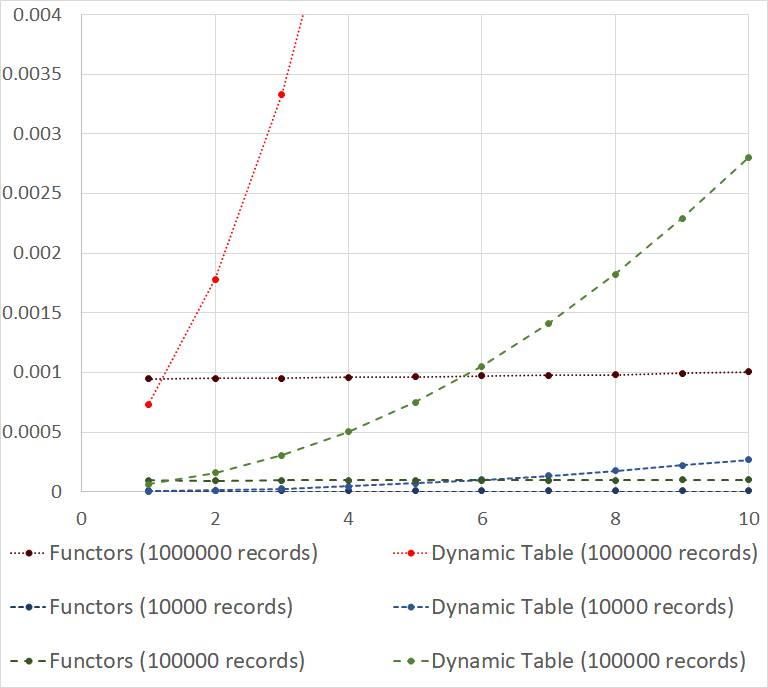
\includegraphics[width = 0.6\textwidth]{Figures/chart}
\end{figure}
\end{frame}

\begin{frame}
\frametitle{Metacasanova}
\framesubtitle{Conclusion}

\textbf{Benefits:}
\begin{itemize}
	\item Significant code reduction.
	\item Performance improvement and static typing with functors.
	\item Fast prototyping and implementation of new languages.
\end{itemize}

\textbf{Problems:}
\begin{itemize}
	\item Programs in the implemented language still need to be expressed in the meta-language.
	\item Performance is worse than a hard-coded implementation of the compiler.
\end{itemize}

\textbf{Future work:}
\begin{itemize}
	\item Use functors to extend Casanova, a DSL for game development, with networking primitives.
	\item Web-based meta-interpreter for a didactic platform to learn programming with interactive feedback. 
\end{itemize}
\end{frame}

\begin{frame}
\centering
\Huge
Thank you!
\end{frame}

\end{document}